\documentclass{beamer}
\beamertemplatenavigationsymbolsempty
\usepackage{lmodern}
\usepackage{helvet}
  \renewcommand{\familydefault}{\sfdefault}
\usepackage{pdfcomment}
    \newcommand{\pdfnote}[1]{\marginnote{\pdfcomment[icon=note]{#1}}}

\mode<presentation>
{
  \usetheme{default}
}

\title{Leadership of Technical Teams}
\author{
  Owen Campbell\\
  \vspace{1cm}
  Twitter: @opcampbell\\
  Google+: OwenCampbell1
}
\date[PyCon UK 2015]{18th September, 2015\\PyCon UK, Coventry}

% \AtBeginSection[]
% {
%   \begin{frame}<beamer>{Outline}
%     \tableofcontents[currentsection]
%   \end{frame}
% }

\begin{document}

\begin{frame}
  \titlepage{}
\end{frame}

{
  \begin{frame}<beamer>{Outline}
    \tableofcontents
  \end{frame}
}

  \section{Introduction}

    \begin{frame}{Introduction}
      Hello World
    \end{frame}


  \section{Authority}

    \begin{frame}{Authority}
    \end{frame}

  \section{Priorities}

    \begin{frame}{Priorities}
    \end{frame}

  \section{Process}

    \begin{frame}{Process}
    \end{frame}

  \section{Style}

    \begin{frame}{Style}
      \begin{figure}
          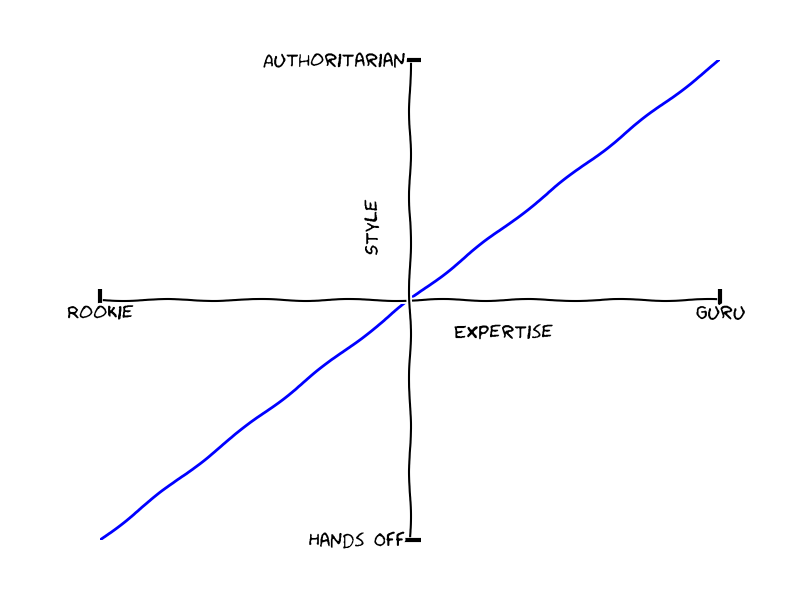
\includegraphics[scale=0.5]{images/style}
        \end{figure}
    \end{frame}

  \section{Conclusion}

    \begin{frame}{Conclusion}
    \end{frame}

    \begin{frame}{Thank You}
      \begin{itemize}
        \item Website: owencampbell.me.uk
        \item Twitter: @opcampbell
        \item Google+: OwenCampbell1
      \end{itemize}
    \end{frame}

\end{document}
